\begin{itemize}
    \item Given the die is fair.
    \item So, for any given throw by A or B:\\
    The probability of getting 6 = $\dfrac{1}{6}$ = p (say)\\
    The probability of NOT getting 6 = $\dfrac{5}{6}$ = q (say)
\end{itemize}
Constraint: A starts the game and A should win.\\
$\implies$ Until A wins, both A and B cannot win.\\
%$\implies$ B(State 2) is absorbing state and it represents the state A loses and B wins.\\
\begin{figure}[!htb]
Corresponding Markov chain is:\\
\begin{center}
    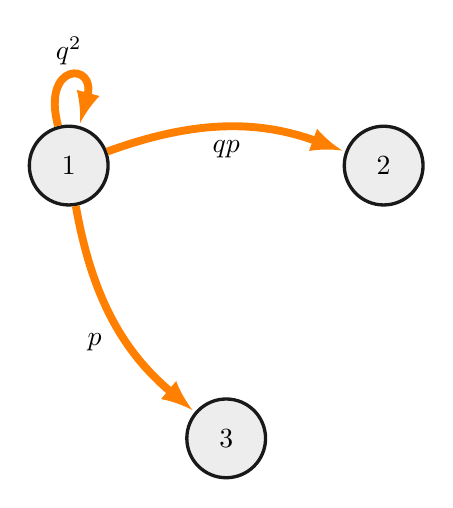
\begin{tikzpicture}[roundnode/.style={circle, draw=black!90, fill=black!7, very thick, minimum size=1cm}]
        \node [roundnode] at (0, 0)     (a)     {1};
        \node [roundnode] at (4, 0)     (b)     {2};
        \node [roundnode] at (2, -3.4641) (w) {3};
        \draw[every loop, auto=right, line width=1mm,
                >=latex, draw=orange,fill=orange]
            (a) edge[bend left=20] node {$qp$} (b)
            (a) edge[loop above=40] node {$q^2$} (a)
            (a) edge[bend right=20] node {$p$} (w);
    \end{tikzpicture}
%        \caption{Modified Markov chain}
        \label{markov/2/fig:Fig1}
\end{center}
\end{figure}
\begin{table}[!htb]
    \begin{center}
    \begin{tabular}{|c|c|}
        \hline
        State & Corresponding description \\
        \hline
        1 & A and B both lose.\\
        \hline
        2 & A loses and B wins.\\
        \hline
        3 & WINNER\\
        \hline
      \multicolumn{2}{c}{Table 1: State description table}
    \end{tabular}
    \end{center}
\end{table}
\begin{definition}
    \vspace{2cm}
    2 and 3 are ABSORBING states.\\
    Transition/Stochastic matrix is: T\\
    \centering
         \text{\small (From)} \begin{blockarray}{ cccc }
                \multicolumn{3}{c}{(\small To)}\\
                & 1 & 2 & 3 \\
                \begin{block}{ c @{\quad} [ @{\,} *{3}{c} @{\,} ] }
                    1 & $q^2$ & qp & p\\ 
                    2 & 0 & 1 & 0\\
                    3 & 0 & 0 & 1\\
                \end{block}
           \end{blockarray} = T
\end{definition}
\begin{theorem}
Every transition matrix can be partitioned as $\mleft(
    \begin{array}{c|c}
        Q & P\\
        \hline
        O & J\\
    \end{array}
    \mright)$\\
    where Q arise from transition probabilities between non-absorbing states\\
    R arises from Transition probability from non-absorbing state to absorbing state.\\
    O = Null matrix,
    J = Identity matrix\\
    $T^k$ approaches $\overline{T}$ as k increases.
    $\overline{T}$ is the limiting matrix and
    $\overline{T} = \myvec{O & NP\\O & J}$\\
    where N is the fundamental matrix.
    $N = (I - Q)^{-1}$\\
    \end{theorem}
\begin{definition}
    The matrix D = NP gives the probability of ending up in the absorbing states (2 and 3) when the chain starts from a non-absorbent state 1.
\end{definition}
\begin{align}
    T = \mleft(
    \begin{array}{c| c c}
        q^2 & qp & p\\
        \hline
        0 & 1 & 0\\
        0 & 0 & 1\\
    \end{array}
    \mright)   \\ 
        Q = \myvec{q^2},
        P = \myvec{qp & p},
        O = \myvec{0 \\ 0},
        J = \myvec{1 & 0\\0 & 1} \label{markov/2/eq:eqn1}
    \end{align}

    \begin{align}
        N = \myvec{1 - q^2}^{-1} = \myvec{\dfrac{1}{1-q^2}}\\
        D = NP = \myvec{\dfrac{qp}{1 - q^2} & \dfrac{p}{1 - q^2}}\\
        \pr{\text{A wins}} = D_2 = \dfrac{p}{1 - q^2} = \frac{\frac{1}{6}}{1 - \frac{25}{36}} = \dfrac{6}{11}
    \end{align}
        \centering
\[
    \pr{\text{A wins}} = \dfrac{6}{11}
\]
OPTION D is correct